\subsection{RiskAdaptive Framework Overview}

The proposed RiskAdaptive framework introduces a risk-aware
intrusion detection architecture for Edge-IoT environments. Unlike
traditional IDS solutions that provide only binary attack
classification, the proposed framework integrates detection with
contextual risk evaluation to prioritize security events based on
their potential impact.

Figure~\ref{fig:architecture} illustrates the overall architecture of
the proposed system. The framework consists of four major components:
data ingestion, intrusion detection, agentic risk analysis, and
security decision support.

\begin{figure}[!t]
\centering
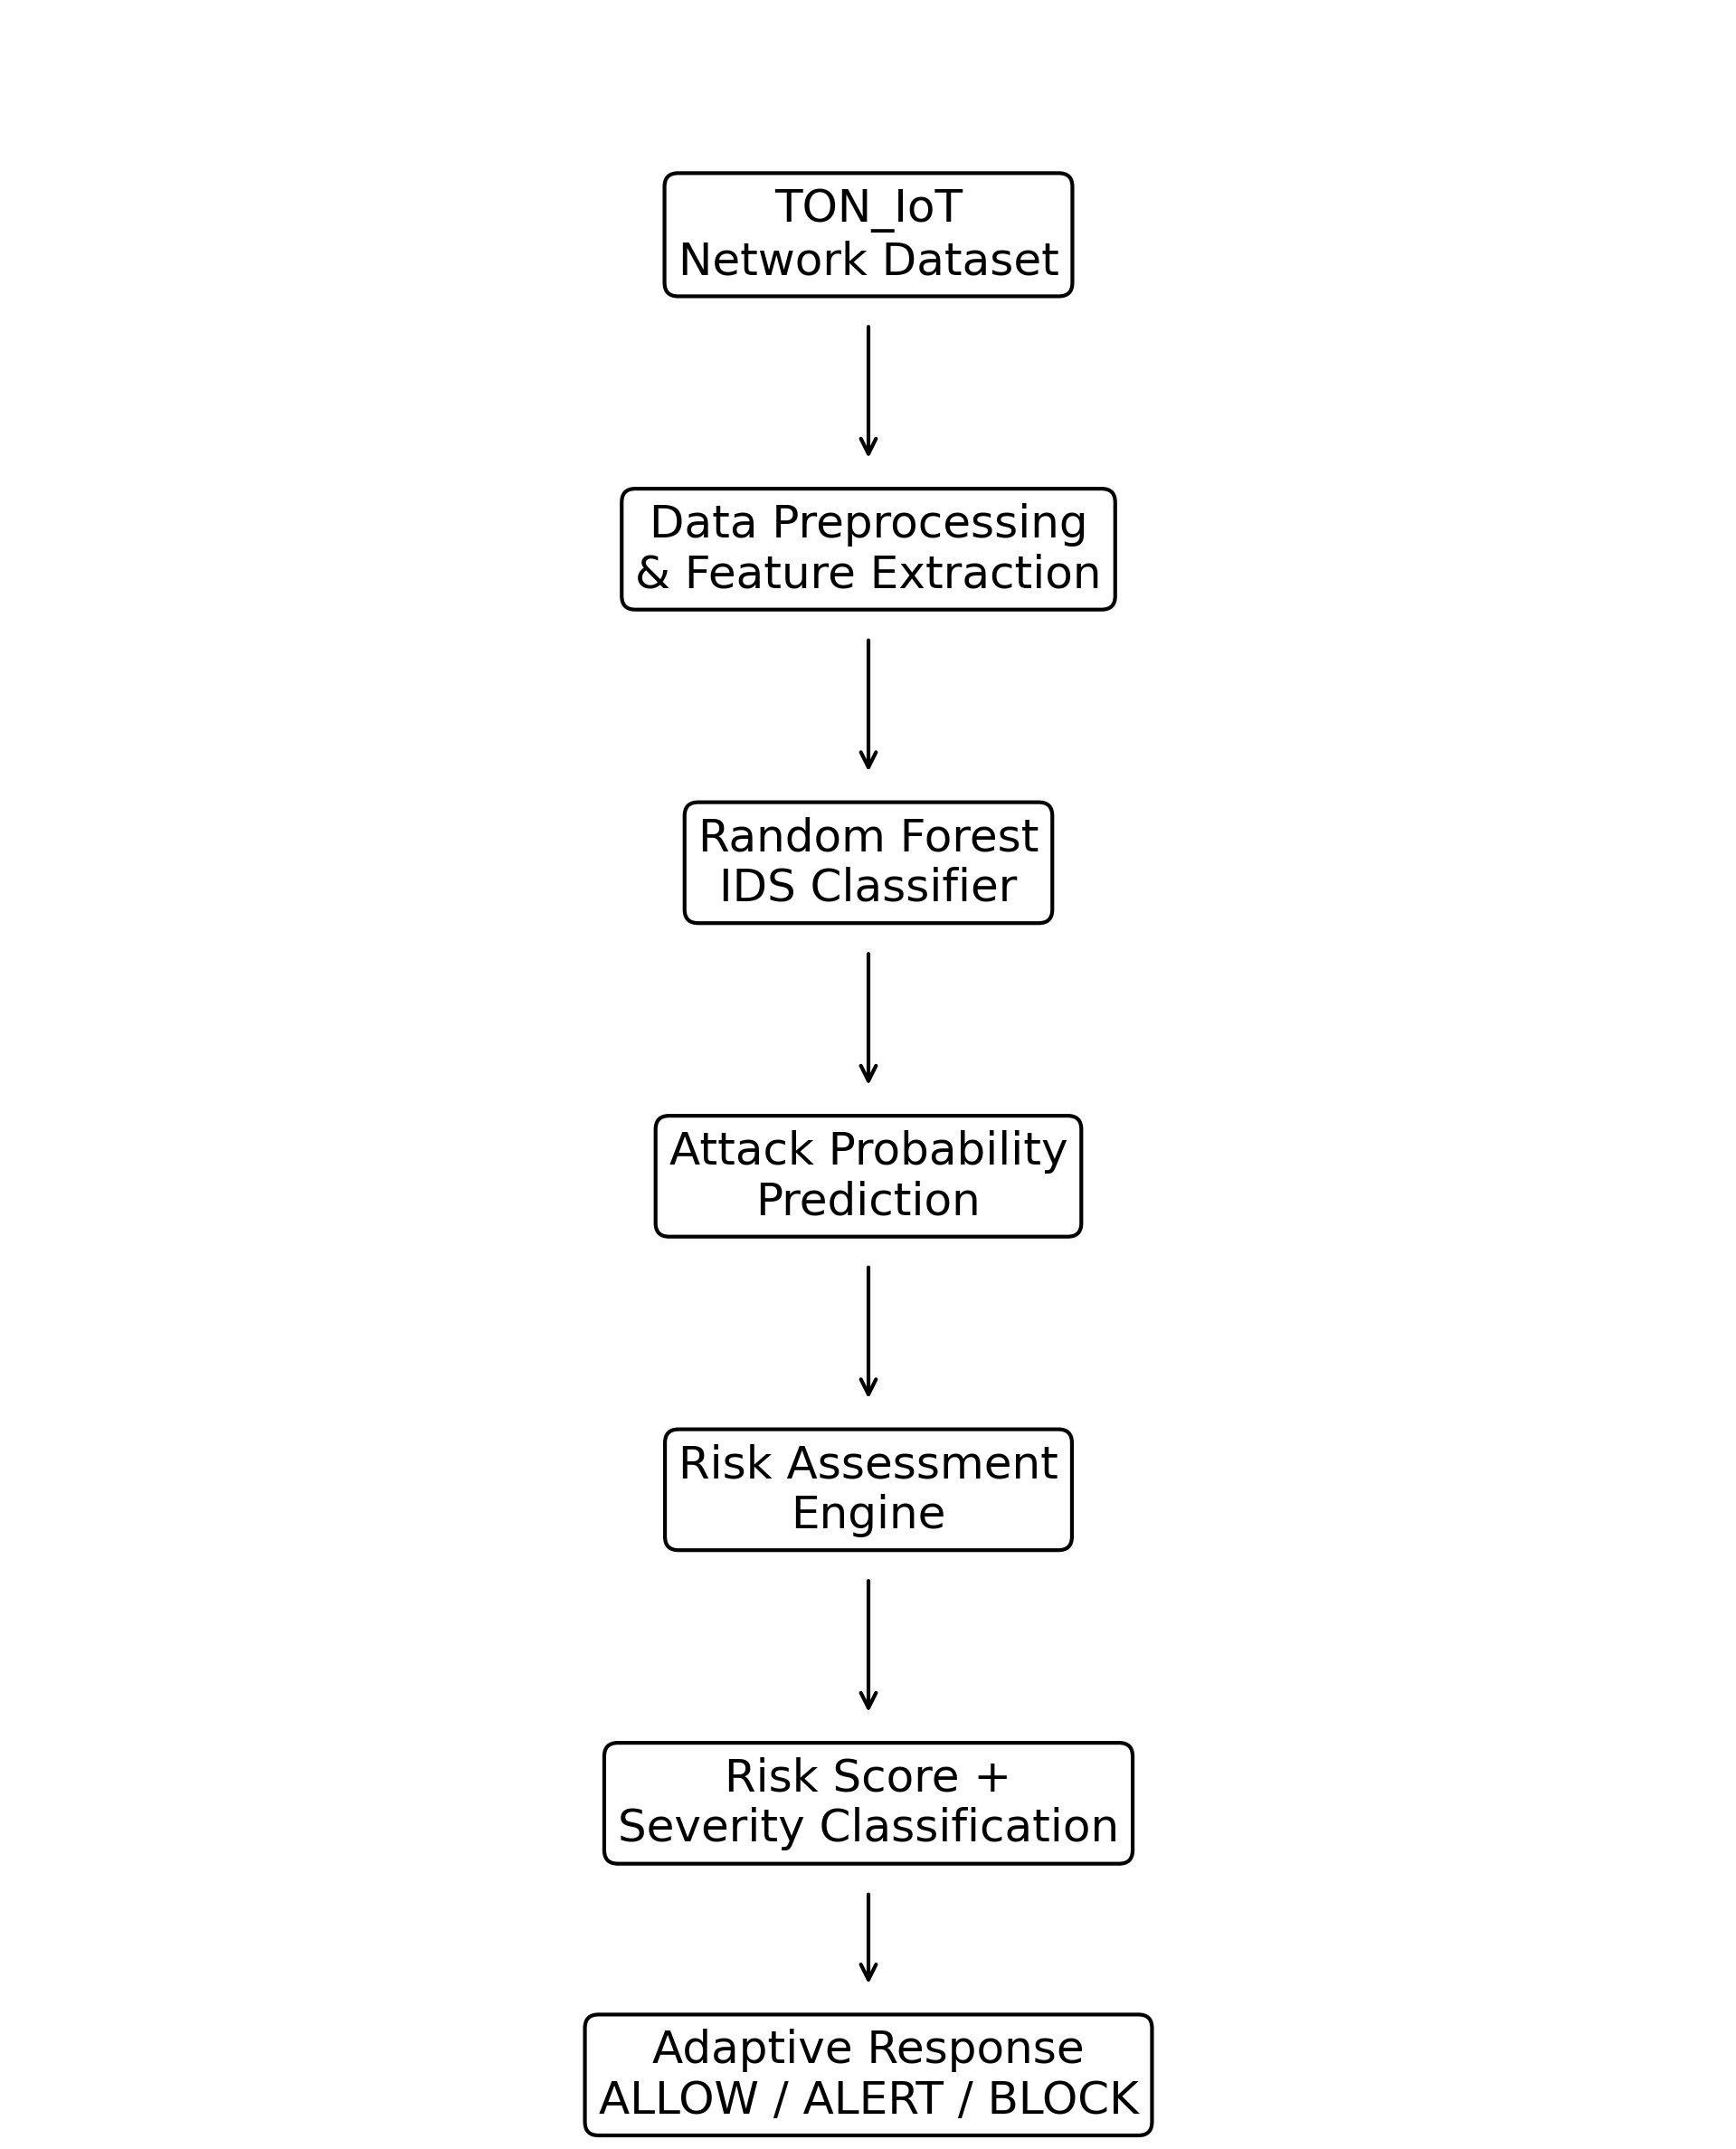
\includegraphics[width=\columnwidth]{figures/riskadaptive_architecture.png}
\caption{Architecture of the proposed RiskAdaptive framework.}
\label{fig:architecture}
\end{figure}


\subsection{Data Processing and Feature Representation}

The framework utilizes network telemetry data obtained from the
\texttt{TON-IoT} dataset. The preprocessing pipeline performs data cleaning,
feature transformation, and preparation of network attributes for
machine learning based classification.

The processed feature representation enables the intrusion detection
model to identify malicious activities while maintaining compatibility
with heterogeneous IoT network environments.


\subsection{Intrusion Detection Module}

The intrusion detection component uses supervised machine learning
classification to distinguish between normal and malicious network
activities. A Random Forest based classifier is employed due to its
ability to model nonlinear relationships among network security
features.

The output of this module consists of the predicted attack category
and associated confidence information, which is forwarded to the
risk assessment layer.


\subsection{Agentic Risk Assessment Engine}

The core contribution of RiskAdaptive is the integration of an
agentic risk evaluation layer above the intrusion detection module.
The risk engine analyzes detected events using contextual security
attributes including attack category, severity level, and potential
impact.

Instead of treating every detected attack equally, the framework
generates a continuous risk score that enables prioritization of
security incidents.


\subsection{Risk Scoring and Severity Classification}

The generated risk score represents the combined impact of detected
security events. Based on predefined risk thresholds, events are
categorized into three severity levels:

\begin{itemize}
\item Low: Minimal security impact requiring monitoring.
\item Medium: Suspicious activity requiring further analysis.
\item High: Critical events requiring immediate attention.
\end{itemize}

This adaptive prioritization mechanism reduces alert overload and
provides security operators with actionable information.


\subsection{Decision Support Workflow}

The final stage converts detection results into security insights by
combining attack identification, risk estimation, and severity
classification. The framework therefore extends conventional IDS
systems from attack detection toward intelligent security
prioritization.
